\section{Marco Teórico}

\subsection{Validación de modelos}
Los modelos son representaciones matemáticas de los mecanismos que rigen los fenómenos naturales \parencite{tedeschi-2006} o como una construcción matemática diseñada para estudiar un sistema del mundo real o fenómeno \parencite{giordano-1997}.\\

\textcite{medina-peralta-2017} indican que la validación de un modelo en la predicción del sistema implica la comparación, por medio de algún método, de las predicciones del modelo con los valores observados del sistema real para determinar su capacidad predictiva.\\

\textcite{mayer-butler-1993}, clasifican los métodos de validación de modelos en Evaluación Subjetiva, Técnicas Visuales, Medidas de Desviación y Pruebas Estadísticas; también señalan que debido a las complejidades y tipos de datos, no existe una combinación establecida de técnicas de validación que sea aplicable en todas las áreas.\\

\textcite{halachmi-2004}, menciona que la validación determina si el modelo matemático es una representación exacta del sistema real, y una forma de validación es comparando los datos reales con los predichos por el sistema.\\

Para la validación de un modelo se evalúan la exactitud y la precisión; la primera se refiere a la proximidad de las predicciones $( z )$  con los valores observados $( y )$, por ejemplo, sus diferencias $ ( d=y-z ) $ del cero y la segunda a la dispersión de los puntos $ (z, y) $; además, en presencia de exactitud la precisión se mide cuantificando la dispersión de dichos puntos respecto a una referencia, por ejemplo, la recta determinística  $ y=x $, o bien, evaluar la varianza de las diferencias $ (\sigma_{D}^{2}) $ alrededor del cero $ (\mu_{D}=0) $ \parencite{medina-peralta-2017}.\\


En la Figura \ref{fig:EsquemaExacPreci} se ilustra la diferencia entre la exactitud y precisión de un modelo de simulación. El caso 1 es inexacto e impreciso, el caso 2 es inexacto y preciso, el caso 3 es exacto e impreciso y el caso 4 es exacto y preciso. En un modelo de predicción lo ideal es que cumpla el caso 4. 

\begin{figure}[H]
	\centering
	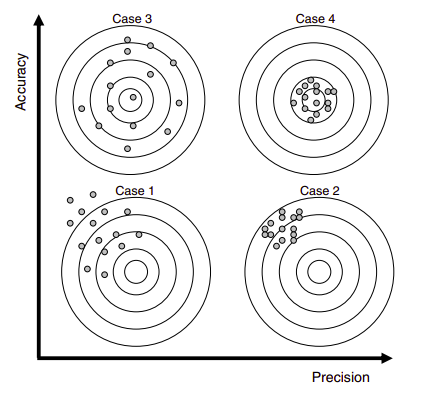
\includegraphics[width=180px]{img/tadeshi_casos.png}
	\caption{Esquematización de Exactitud y Precisión. Fuente: \textcite{tedeschi-2006}.}
	\label{fig:EsquemaExacPreci}
\end{figure}
\FloatBarrier

De manera similar, la Figura \ref{fig:ComparmedidExacPreci} representa los conceptos ilustrados en la Figura \ref{fig:EsquemaExacPreci} en una forma numérica; el eje $X$ y el eje $Y$ representan al modelo de los valores predichos contra los observados respectivamente. El caso 1 es inexacto e impreciso, el caso 2 es inexacto y preciso, el caso 3 es exacto e impreciso y el caso 4 es exacto y preciso. La línea punteada representa la línea de $X = Y$ . En un modelo de predicción lo ideal es que cumpla el caso 4. 

\begin{figure}[H]
	\centering
	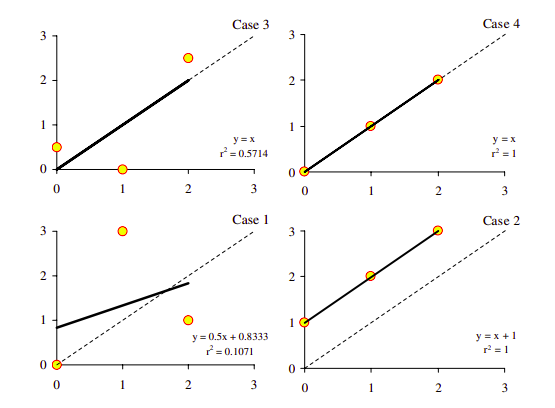
\includegraphics[width=0.6\linewidth]{img/tedeshi_casos_2.png}
	\caption{ Comparación de las medidas de Exactitud y Precisión. Fuente: Tedeschi (2006).}
	\label{fig:ComparmedidExacPreci}
\end{figure}
\FloatBarrier

Las estimaciones del intercepto y la pendiente son buenos indicadores de la exactitud: cuanto mas cerca
estén simultáneamente de cero y uno respectivamente mayor es la exactitud. La estimación del coeficiente de
determinación $(R^{2})$ es un buen indicador de la precisión: cuanto mayor es la $R^{2}$ mayor es la precisión \parencite{balam-2012}.\\

Por su parte, \textcite{mayer-butler-1993} indican que la prueba $t$ paramétrica de medias y el análisis de regresión lineal de la grafica observada frente a la predicha son los métodos estadísticos generales mas útiles, sin embargo, cada método inferencial se encuentra principalmente sujeto a las dificultades para satisfacer sus supuestos.\\



\subsection{Regresión lineal simple}
Una de las técnicas mas comunes en la validación de modelos es la de Regresión Lineal Simple de los observados sobre los predichos \parencites{analla-1998, mayer-1994, tedeschi-2006}.\\

El análisis de regresión lineal tiene como objetivo modelar en forma matemática el comportamiento de una variable de respuesta en función de una o mas variables independientes \parencite{gutierrez-2012}. Por lo tanto, se ajusta el modelo  $ y_{i} = \beta_{0} + \beta_{1}z_{i} +\epsilon $ donde $ 1 \leq i \leq n$, $ y_{i}$ es el valor real observado en la $i$-ésima unidad experimental, $ z_{i}$ es el correspondiente valor predicho por el modelo a validar, $\epsilon_{i}$ es el componente aleatorio o error, $\beta_{0}$ es la ordenada al origen y $\beta_{1}$ la pendiente \parencite{zacarias-2023}.\\

Esta técnica se encuentra principalmente sujeta al cumplimiento de sus supuestos. Cuando los residuales son independientes, se ajustan a una distribución normal y tienen varianza común, se aplican pruebas de hipótesis estadísticas para evaluar la exactitud, intercepto cero y pendiente uno, ya sea mediante pruebas t de Student, o bien, mediante una prueba F para determinar si el intercepto y la pendiente son simultáneamente cero y uno respectivamente \parencite{balam-2012}.


\subsubsection{Verificación de los supuestos de normalidad, varianza constante e independencia para los residuales de un modelo de regresión}

\vspace{.8cm}

\textbf{Supuesto de normalidad}\\

Para la verificación del supuesto de normalidad de los residuales $\epsilon_i$ del modelo de regresión se requiere una muestra de los residuales $e_1, e_2, \cdots, e_n$ y de su distribución empírica:\\


\begin{center}
	$$\hat{F}(x)=\frac{\sum_{i=1}^n I_{(- \infty,x)}(e_i)}{n}  \;\; \forall \;\; x \;\; \in \Re.$$
\end{center}

Se contrastan las siguientes hipótesis:\\

$H_0:$ Los $\epsilon_i$ tienen distribución normal vs. $H_a:$ Los $\epsilon_i$ no tienen distribución normal.\\

El estadístico de Shapiro-Wilk es uno de los más consolidados y con mayor potencia estadística entre las estadísticas existentes \parencite{arcone-2006}; este estadístico ha demostrado de manera general, resultados adecuados en comparación a las pruebas clásicas \parencite{arcone-2006}, pero especialmente cuando se trabaja con distribuciones de colas cortas \parencite{thadewald-2007} y con un tamaño muestral inferior a 30, ya que muestra una alta variabilidad cuando se modifican tanto la simetría como el tamaño muestral de la distribución, especialmente entre 20 y 50 datos \parencite{yazici-2007}.\\

La estadística de \textcite{Lilliefors-1967} consiste en una mejora de la estadística de Kolmogorov- Smirnov (K-S), sustentada sobre los mismos principios estadísticos, pero específica para aquellos casos en donde la media y la varianza son desconocidas. De este modo, se evita el efecto que provoca, como ocurre en el caso de K-S, la estimación de los parámetros de la muestra \parencite{steinskog-2007} y se recomienda, por tanto, como el estadístico más apropiado para dichos casos \parencite{oztuna-2006}; esta estadística está indicada para muestras grandes.\\


\textbf{Estadístico de Shapiro-Wilk}


\begin{center}
 $$SW=\frac{1}{^{max}_{i\leq i \leq n} \mid \Phi (e_i) \mid}[\sum_{i=1}^k a_i(e_{(n-i+1)-e_(i)})]^2$$
\end{center}


Donde:\\
$\Phi (x) =$ Es la función acumulada de la distribución Normal Estándar.\\
$k =$ Es el menor de los enteros mayor o igual a $n/2$.\\
$a_i =$ Coeficientes que son calculados para un tamaño de muestra $n$ y se obtienen de la tabla A17: Coeficientes de la prueba de Shapiro-Wilk \parencite{conover-1999}.\\
$e_{(i)} =$ Es el $i$-ésimo menor de la muestra $e_1, e_2, \cdots , e_n$.\\\\
Se rechaza la hipótesis de normalidad $H_0$ con nivel de significancia $\alpha$ si $SW$ es mayor que el cuantil $W_{\alpha}$ correspondiente al tamaño de muestra $n$ y al nivel de significancia $\alpha$ proporcionado en la tabla A17 \parencite{conover-1999}, o bien, si $p-valor \leq \alpha$.\\



\textbf{Estadístico de Lilliefors}

\begin{center}
	$$D = ^{max}_{1\leq i \leq n}\lbrace ^{max}_{1\leq i \leq n} \lbrace \frac{1}{n} - \Phi (e_{(i)}) \rbrace , ^{max}_{1 \leq i \leq n} \lbrace \Phi (e_{(i)}) - \frac{i-1}{n} \rbrace   \rbrace$$
\end{center}



Donde:
$\Phi (x) =$  Es la función acumulada de la distribución Normal Estándar.\\
$e_{(i)} =$ Es el $i$-ésimo menor de la muestra $e_1, e_2, \cdots , e_n$.\\

Se rechaza a hipótesis de normalidad $H_0$ con nivel de significancia $\alpha$ si $D$ es mayor que el cuantil $D_\alpha$ correspondiente al tamaño de muestra $n$ y al nivel de significancia $\alpha$ proporcionado en la tabla A.19(a), A.19(b), o bien, A.19(c) de \textcite{daniel-1990} dependiendo si únicamente $E(\epsilon)$ es desconocida, sólo $\sigma ^2$ o ambos parámetros son desconocidos, o bien, si $p-valor \leq \alpha$. El supuesto de normalidad también se verifica con el gráfico de probabilidad normal, si los puntos en dicha gráfica mantienen una forma semejante a una línea recta, entonces el supuesto de normalidad se cumple.\\



\textbf{Supuesto de varianza constante}\\\\
Para la verificación del supuesto de varianza constante en los residuales $\epsilon_i$, se requiere una muestra de los residuales $e_1, e_2, \cdots , e_n$ y se contrastan las siguientes hipótesis:\\

$H_0: V(\epsilon_i) = V(\epsilon_j) \;\; \forall \;\; i \neq j$   vs.   $H_a: V(\epsilon_i) \neq V(\epsilon_j)$ para alguna $i \neq j$. \\

Existe una variedad de pruebas estadísticas que contrastan hipótesis semejantes y que permiten evaluar el supuesto de homocedasticidad, las pruebas más utilizadas son la de Breusch-Pagan, la de White, la de Score \parencite{taboga-2017}, la de Goldfeld-Quandt \parencite{goldfeld-2024} y la de Harrison-McCabe \parencite{harris-1979} .\\

A continuación, se describen las pruebas de Breusch-Pagan y la de White.\\




\textbf{Prueba de Breush-Pagan} ~\parencites{breush-1979, verbeek-2004}\\

La prueba de Breusch-Pagan sólo detecta formas lineales de heterocedasticidad; por lo que consiste en ajustar el modelo de regresión lineal entre los residuales al cuadrado y las variables independientes:

\begin{center}
	$${e_i} ^2=\delta _0 + \delta _1 X_1+ \cdots + \delta _k X_k  + u \; .$$
\end{center}

Se contrastan las hipótesis:\\

\begin{center}
	$H_0: \delta _0 = \delta _1 = \cdots =\delta _k=0 $  vs.  $H_a: \delta_i \neq 0$ para alguna $i$.
\end{center}


En $H_0$ se establece que los residuales no son función de las covariables del modelo; el estadístico de prueba está dado por:


\begin{center}
	$$B=n R ^2 \sim \chi_k ^2 \; ,$$
\end{center}


donde $R^2$ es el coeficiente de determinación del modelo de regresión en ${e_i} ^2=\delta _0 + \delta _1 X_1+ \cdots + \delta _k X_k  + u$ y la estadística $B$ se distribuye asintóticamente Ji-cuadrada con $k$ grados de libertad.\\

Si el estadístico de prueba $B$ tiene un valor $p-valor$  por debajo del valor $\alpha$ establecido, entonces se rechaza la hipótesis nula de homocedasticidad y se asume heterocedasticidad; esta prueba solo detecta formas lineales de heterocedasticidad. Algunos autores (incluidos \textcite{bickel-1978} y \textcite{koenker-1981}) han sugerido que la prueba estadística de Breusch-Pagan puede no ser precisa para datos no normales.\\


\textbf{Prueba White} ~\parencite{verbeek-2004} \\

A diferencia de la prueba de Breush-Pagan que sólo detecta formas lineales de heterocedasticidad, la prueba de \textcite{white-1980} permite contrastar no linealidades, ajustando un modelo de regresión lineal entre los residuales al cuadrado y los productos cruzados de todos los regresores:


\begin{center}
	$${e_i} ^2=\delta _0 + \delta _1 X_1+ \cdots + \delta _{k} X_k + \delta _{k+1} X_1 X_2+ \cdots +\delta _l X_{k-1} X_k+  \delta _{l+1} X_1 ^2 + \cdots  + \delta _{l+k} X_k ^2 + u(i) \; , $$
\end{center}


donde {\large $l=\frac{k(k-1)}{2}$}.\\ \\
Se contrastan las hipótesis:\\
$H_0: \delta _1 =  \cdots =\delta _k=\delta _{k+1} =  \cdots =\delta _l= \cdots=\delta_{l+k} =0 $  vs.  $H_a: \delta_i \neq 0$ para alguna $i$.\\

El estadístico de prueba dado por:

\begin{center}
	$$W=n R^2 \sim \chi_r ^2 \; ,$$
\end{center}


donde $R^2$ es el coeficiente de determinación del modelo de regresión en (i); y la estadística $W$ se distribuye asintóticamente Ji-cuadrada con $r=(3k + k^2)/2$ grados de libertad. Si el estadístico de prueba $W$  tiene un valor p-valor por debajo del valor $\alpha$ establecido, entonces se rechaza la hipótesis nula de homocedasticidad y se asume heterocedasticidad.\\


La prueba de White es extremadamente general y su potencia puede ser bastante baja frente a ciertas alternativas, particularmente si el número de observaciones es pequeño; en esta prueba se relaja la suposición de normalidad. \\

El supuesto de homocedasticidad también se verifica mediante el grafico de dispersión entre los valores predichos  contra los residuales; y se utiliza el siguiente criterio:\\

\begin{itemize}
	\item[a)] Si los puntos forman algo similar a un cono o embudo, la varianza no es constante.
	
	\item[b)] Si los puntos sugieren algún patrón, no se asegura que la varianza sea constante.
	
	\item[c)] Los puntos permanecen dentro de una banda horizontal (sugeridas por los datos), o bien, los puntos se encuentran en posiciones al azar, se dice que la varianza es constante. \\
\end{itemize}



\textbf{Supuesto de independencia}\\

Para la verificación de este supuesto se contrastan las hipótesis:\\

$H_0:\;$ Los $e_i$ no están correlacionados vs. $H_1:\;$ Los $e_i$ sí están correlacionados.\\

Los estadísticos más utilizados para contrastar estas hipótesis son el de Durbin-Watson y el de Breusch-Godfrey. Si no se rechaza la hipótesis $H_0$ para un nivel de significancia $\alpha$ se dice que se cumple este supuesto. La verificación de este supuesto también se realiza con el gráfico de dispersión entre el orden de entrada de los datos y los residuales; si en este gráfico es posible identificar alguna relación entre el orden de entrada y los residuales, se dice que el supuesto de independencia no se cumple, mientras que, si se observa que los puntos están distribuidos al azar, esto indica que hay independencia entre los residuales.


\subsubsection{Validación de modelos con la técnica de regresión lineal simple \parencite{febles-2014}}

\textcite{febles-2014}, describe la validación de modelos con la técnica de regresión lineal simple que se centra en determinar el grado de exactitud y precisión del modelo basándose en el trabajo previo de \textcite{balam-2012}.\\

Sea un modelo $Y = H(\Theta )$, con una muestra pareada $(z_{1}, y_{1}), (z_{2}, y_{2}) , \dots , (z_{n}, y_{n})$ de valores observados y predichos respectivamente por el modelo. Bajo estas condiciones, se considera el modelo de regresión lineal: $y_{i}= \beta_{0} + \beta_{1}z_{i}$, donde $ 1 \leq i \leq n$. Donde  los estimadores de mínimos cuadrados para $\beta_{0}$,  $\beta_{1}$ y el coeficiente de determinación $R^{2}$ son respectivamente: \\

\begin{center}
{\large$\hat{\beta_{0}} = \hat{y} - \hat{\beta_{1}} \bar{z}$} ,\\
\end{center}

\begin{center}
{\Large$ \hat{\beta_{1}} = \frac{\sum_{i=1}^{n} (z_{i} - \bar{z} ) (y_{i} - \bar{y})} {  \sum_{i=1}^{n} (z_{i} - \bar{z} )^{2} }$} , \\
\end{center}

\begin{center}
{\Large $R^{2} = \frac{ \sum_{i=1}^{n} ( \hat{y}_{i} - \bar{y})^{2}} { \sum_{i=1}^{n} ( y_{i} - \bar{y})^{2}  }$ }  y  $ 0 \leq R^{2} \leq 1$,
\end{center}


donde $ \bar{z}$ y $ \bar{y}$ son las medias muéstrales de los valores observados y predichos respectivamente por el modelo; la evaluación estadístico de la exactitud y precisión depende del cumplimiento de los supuestos de normalidad y de varianza constante de los errores i en el modelo. \\


Los residuales $\epsilon_{i} = y_{i} - \bar{y}_{i}$ son estimaciones de los errores $i$ en el modelo, verificando el  supuesto de normalidad en los residuales $\epsilon_{1}, \epsilon_{2} , \dots, \epsilon_{n} $, con pruebas de bondad de ajuste, como la de Kolmogorov-Smirnov y Shapiro Wilk. El supuesto de varianza constante se verifica con el grafico de dispersión entre los predichos $y_{i}$ y los residuales $\epsilon_{i}$ del modelo. Con todas las combinaciones de los supuestos de normalidad y varianza constante, la evaluación de la exactitud y precisión del modelo $Y = H(\Theta )$ se analizan en los siguientes tres casos: cuando la muestra de residuales es independiente con distribución normal y varianza constante (NVC); cuando la muestra de residuales es independiente con distribución no normal y varianza constante (NNVC) y cuando la muestra
de residuales es independiente con varianza no constante (NVD - NNVD).

\subsubsection{Evaluación de la exactitud de un modelo}

Cuando se cumplen los supuestos de la Regresión, la verificación de la exactitud de un modelo puede llevarse a cabo vía dos pruebas t de Student, o bien, mediante una prueba F \parencite{balam-2012}.\\

La Prueba F Conjunta que considera el intercepto y la pendiente de manera conjunta, ambos valores agrupados en un vector de dimensión dos, a diferencia del caso anterior, se compara que el vector de parámetros  sea  contra que no lo sea. Bajo la premisa de que los residuales del modelo entre los observados y predichos cumplen los supuestos de normalidad y varianza constante,la prueba de hipótesis conjunta permite obtener una región de confianza para el vector de parámetros ,en este caso,se dice que el modelo ese exacto cuando la región de confianza conjunta contiene al punto $(0,1)$. \parencite{zacarias-2023}.\\

Para la aplicación de la F conjunta se ajusta el modelo de regresión lineal a simple con los supuestos de que los residuos ajustados se distribuyan normal, son independientes y tienen varianza constante \parencite{ayala-2024}.\\

La Prueba F Conjunta considera un sólo procedimiento que nos permite establecer si un modelo es exacto considerando simultáneamente el intercepto \(\beta_0\) y la pendiente \(\beta_1\), es decir, se prueba estadísticamente si  {\Large $\bigl(\begin{smallmatrix} \beta_{0} \\ \beta_{1} \end{smallmatrix}\bigr) = \bigl(\begin{smallmatrix}0  \\  1\end{smallmatrix}\bigr) $} \parencite{zacarias-2023}.\\

\textcite{zacarias-2023}, para evaluar la exactitud de un modelo ante los escenarios NNVC, NVD y NNVD, implemento un método que consiste en estimar la distribución de la estadística F a través de muestras Bootstrap robustas propuestas en \textcite{rana-2012}, en donde dependiendo del caso que se presente se implementan los distintos tipos de remuestreo propuestos por \textcite{wu-1986} y \textcite{liu-1988} y a partir de estas construir una región de confianza para el vector de parámetros $ \mathbf{\beta} = (\beta_{0}, \beta_{1})$.\\


\subsubsection{Evaluación de la precisión de un modelo}

\textcite{zacarias-2023}, menciona que una parte importante del método de regresión lineal, es que estudia si dicha relación permite realizar estimaciones con una precisión aceptable; por lo que también se considera como un criterio cuantitativo relevante para evaluar la calidad de ajuste de la regresión, el coeficiente de determinación $R^{2}$, que en general se interpreta como la proporción de la variabilidad en los datos observados $y_{i}$, que es explicada por el modelo.\\


\textcite{balam-2012}, utilizó un intervalo de confianza Bootstrap para medir la precisión de un modelo, donde el esquema de remuestreo propuesto depende del cumplimiento o no del supuesto de varianza constante. Cuando se cumple dicho supuesto se emplea un intervalo de confianza Bootstrap de residuales balanceado por el método Percentil con sesgo corregido acelerado para evaluar la precisión de un modelo; y cuando no se cumple el supuesto de varianza constante se emplea un intervalo de confianza Bootstrap pareado balanceado por el método Percentil con sesgo corregido acelerado.\\

\subsubsection{El coeficiente de determinación $R^{2}$}

El coeficiente de determinación $R^{2}$ se utiliza cuando las variables de estudio son cuantitativas y están medidas en una escala de intervalo o razón, siendo una herramienta común para medir el ajuste del modelo a los datos. El valor de $R^{2}$
se interpreta frecuentemente como la proporción de la variación de la variable dependiente explicada por el modelo de regresión lineal simple \parencite{balam-2012}. Sin embargo, es importante señalar que $R^{2}$
presenta varias limitaciones y características que deben ser tomadas en cuenta al evaluar su utilidad.\\


Según lo señalado por \textcite{balam-2012}, algunos puntos clave sobre $R^{2}$:\\

\begin{enumerate} 
	\item $R^{2}$ no mide la magnitud de la pendiente de la recta de regresión ajustada, ni implica que una pendiente grande se corresponda con un valor grande de $R^{2}$. 
	
	\item Es posible obtener un valor grande de $R^{2}$ agregando términos adicionales al modelo, lo que puede no reflejar una mejora real en la calidad del modelo.
	
	\item El valor de $R^{2}$  no mide adecuadamente la relación entre las variables si no existe una relación lineal, por lo que puede ser grande aunque 
	y no tengan una relación lineal significativa. 
	
	\item Un valor elevado de $R^{2}$ no necesariamente implica que el modelo sea un buen predictor, ya que puede estar influenciado por factores no realistas en los datos.
	
	\item En algunos casos, $R^{2}$ puede ser pequeño si el intervalo de las $z$  es demasiado estrecho para detectar una relación significativa con $y$. 
	
	\item En presencia de valores atípicos o agrupamientos (clustering) en los datos, $R^{2}$ puede ser engañoso, pues un valor grande podría ser el resultado de estos factores, en lugar de un ajuste verdadero. \\
\end{enumerate}


A pesar de sus limitaciones,  $R^{2}$ tiene ciertas ventajas, como cuando su valor es cercano a cero, lo que indica que el modelo no se ajusta bien a los datos. Sin embargo, si no hay puntos repetidos, es posible construir un modelo polinómico de grado $n-1$ que ofrezca un ajuste perfecto, lo que también pone en evidencia la necesidad de interpretar  $R^{2}$ con cautela.\\

Entre otras características, se destaca que el valor esperado de  $R^{2}$ puede aumentar o disminuir dependiendo de la variabilidad de la variable independiente $z$, y que, debido a la falta de conocimiento sobre su distribución exacta,  $R^{2}$  no debe usarse para hacer predicciones directas.\\


Dadas estas limitaciones, es importante considerar estudios adicionales que profundicen en las propiedades de $R^{2}$. \textcite{Ohtani-2004}, mencionan que para medir la precisión de un modelo de regresión lineal simple, al utilizarse tradicionalmente el coeficiente de determinación  \( R^2 \) y el coeficiente de determinación ajustado, se han presentado estudios sobre las propiedades de muestras pequeñas de \( R^2 \) y \( \overline{R}^2 \) como lo son \textcite{barten-1962} que sugiere una versión modificada de \( R^2 \) para reducir su sesgo, y la propuesta de \textcite{crammer-1987} al derivar las fórmulas exactas para los dos primeros momentos de \( R^2 \) y \( \overline{R}^2 \), quien muestra que \( R^2 \) está seriamente sesgado hacia arriba en muestras pequeñas, mientras que \( \overline{R}^2 \) es más inestable que \( R^2 \) en términos de desviación estándar.\\


Por lo cual, en \textcite{Ohtani-2004} deriva las fórmulas exactas para la función de densidad, la función de distribución y el momento \(m\)-ésimo, realizando un análisis numéricos basados en las fórmulas exactas, todo esto considerando un modelo de regresión lineal donde los términos de error obedecen a una distribución \(t\) multivariada, examinando los efectos del alejamiento de la normalidad de los términos de error en las distribuciones exactas de \(R^2\) y \(\bar{R}^2\). Con intervalos de confianza de \(R^2\) y \(\bar{R}^2\), muestran que el sesgo hacia arriba de \(R^2\) se vuelve significativo y que el error estándar de \(R^2\) aumenta a medida que los grados de libertad de la distribución de error \(t\) multivariada (\(\nu_0\)) disminuyen. También se muestra que, cuando los valores de \(\nu_0\) y el coeficiente de determinación de la población (\(\Phi\)) son pequeños, los límites superiores de confianza de \(R^2\) y \(\bar{R}^2\) son muy grandes.\\

Adicionalmente, \textcite{christou-2005} explica la distribución del coeficiente de determinación muestral en el caso de regresión simple utilizando su relación con la distribución \(F\) no central. Introduce el concepto de coeficiente de determinación verdadero, el cual es útil en estudios de simulación donde la varianza del término de error es conocida, permitiendo construir relaciones con una fuerza predeterminada.\\







\subsection{Regresión lineal robusta}
En un modelo de regresión lineal, los supuestos de normalidad y homocedasticidad son fundamentales para garantizar la validez de los estimadores obtenidos por mínimos cuadrados ordinarios (OLS). Sin embargo, en la práctica, estos supuestos rara vez se cumplen debido a la presencia de valores atípicos, heterocedasticidad o discrepancias en las hipótesis del modelo. En estos casos, los estimadores de regresión robusta se presentan como una alternativa confiable, ya que están diseñados para ser menos sensibles a dichas anomalías y proporcionar inferencias más confiables sobre los parámetros del modelo \parencite{zacarias-2023}.\\

\textcite{annalisa-2024}, menciona que la regresión robusta ofrece ventajas significativas frente a métodos como la regresión ponderada basada en mínimos cuadrados iterativamente reponderados (IRWLS), especialmente en contextos con patrones heterocedásticos en los residuos. No solo permite gestionar de manera óptima los valores atípicos, sino que también proporciona un enfoque más eficaz para manejar la heterocedasticidad y las desviaciones de los supuestos clásicos del modelo.\\


El objetivo principal de la regresión robusta es desarrollar métodos que produzcan estimaciones precisas y resistentes a influencias indebidas en los datos. Una de las métricas clave para evaluar la robustez de un estimador es el punto de ruptura, definido como la mínima fracción de datos atípicos necesarios para invalidar completamente el estimador. Mientras que los estimadores clásicos como OLS tienen un punto de ruptura bajo que converge a cero a medida que aumenta el tamaño de la muestra, los estimadores robustos modernos pueden alcanzar un punto de ruptura de hasta el 50\%, lo que los hace altamente resistentes ~\parencites{siegel-1982,rousseeuw-1984}. \\

Entre los estimadores robustos más avanzados se encuentra el MM-Estimador, introducido como una combinación de alta eficiencia y robustez.El MM-Estimador es especialmente útil en contextos donde los datos contienen una proporción significativa de valores atípicos, ya que logra una eficiencia asintótica superior al 85\% y un punto de ruptura máximo del 50\% \parencite{rousseeuw-yohai-1984}. Este balance lo convierte en una herramienta clave para análisis estadísticos robustos, asegurando un ajuste confiable incluso en condiciones adversas.\\



\subsubsection{MM-Estimador \parencite{yohai-1987}}
El estimador MM tiene las siguientes propiedades: (i) es altamente eficiente cuando los errores tienen una distribución normal y (ii) su punto de ruptura es 0.5.\\

El estimador MM se define en un procedimiento de tres etapas. En la primera etapa, se calcula una estimación de regresión inicial que es consistente, robusta y con un alto punto de ruptura, pero no necesariamente eficiente. En la segunda etapa, se calcula un estimador M de la escala de errores utilizando residuos basados en la estimación inicial. Finalmente, en la tercera etapa se calcula un estimador M de los parámetros de regresión basada en una función $\psi$ descendente.\\

Considerando el modelo de regresión lineal simple:
\begin{center}
$y_{i}= \beta_{0} + \beta_{1}z_{i}$, $1 \leq i \leq n, $
\end{center}

\textcite{huber-1981} define los estimadores M de la siguiente manera: Sea una función real que satisfaga los siguientes supuestos (A1):

\begin{enumerate}[label=\roman*.]
	\item $\rho(0) = 0$.
	\item   $\rho(-u) =  \rho(u)$.
	\item $1 \leq i \leq v$ implica $\rho(u) \leq  \rho(v)$.
	\item $\rho$ es continua.
	\item Sea a = sup $\rho(u)$, entonces $0<a< \infty$.
	\item Si $\rho(u) < a $ y $0 \leq  u < v $, entonces  $\rho(u) <  \rho(v)$.
\end{enumerate}

Dada una muestra de tamaño $n$, $ \mathbf{u} = (u_{1}, u_{2}, \dots , u_{n})$,  el estimador M, $s(\mathbf{u})$ está de nido como el valor de $s$ que es la solución de\\

\begin{center}
	{\Large	$\frac{1}{n} \sum_{i=1}^{n} \rho( \frac{u_{i}}{s}) = b$ },\\
\end{center}

donde $b$ puede de definirse como $E_{\Phi}(\rho(u)) = b$, donde $\Phi$ denota la distribución normal estándar.\\

Se cumple que si $c(\mathbf{u}) = \#\{i : 1 \leq i \leq n, u_{i}=0\} / n < 1- (b/a) $, entonces la sumatoria previa tiene solución única y esta solución es diferente de 0. Si $c(\mathbf{u}) \geq 1 -  (b/a)$, se define $s(\mathbf{u}) = 0$. \\

Luego, el estimador MM se define en tres etapas de la siguiente manera:\\

\begin{enumerate}
	\item Sean $ \beta_{0}^{'}$ y $ \beta_{1}^{'}$ estimaciones de los parámetros $\beta_{0}$ y $ \beta_{1}$ respectivamente con un alto punto de ruptura, posiblemente 0.5.
	\item  Calcular los residuales\\
	\begin{center}
		 $ \epsilon_{i} = y_{i} -\beta_{0}^{'} -\beta_{1}^{'} z_{i}  $, $1 \leq i \leq n $\\
	\end{center}
	
	y calcular $s_{n} = s(\epsilon_{i})$, el estimador M definido previamente, usando una función $\rho_{0}$ que satisface los supuestos (A1) y considerando una constante $b$ tal que $b/a = 0.5$, donde$ a = $ máx $ \rho_{0}(u)$, lo cual implica que para esta escala la estimación tiene un
	punto de ruptura igual a 0.5.
	
	\item  Sea $\rho_{1}$ otra función que satisfaga los supuestos (A1) y tal que\\
	\begin{center}
		$\rho_{1}(u) \leq \rho_{0}(u)$ y\\
		sup $\rho_{1}(u)$  = sup $ \rho_{0}(u) = a$.\\
	\end{center}

	
	Sea $\psi_{1} = \rho_{1}^{'}$. Entonces el estimador MM, se define como cualquier solución de\\
	\begin{center}
	{\large	$\sum_{i=1}^{n} \psi_{1} (\frac{\epsilon_{i}}{s_{n}}) z_{i} = 0$}\\
	\end{center}

\end{enumerate}


\subsubsection{ Algoritmo de MM-Estimador \parencite{zacarias-2023} }
Como se presenta en la tesis de \textcite{zacarias-2023}, el algoritmo MM-Estimador es un enfoque robusto que mejora la estimación de los coeficientes en presencia de valores atípicos. A continuación, se describe el algoritmo:\\

Sea\\
\begin{center}
 $ y_{i} = \beta_{0} -\beta_{1}z_{i} + \epsilon_{i} $, $1 \leq i \leq n $,\\
\end{center}

una muestra de tamaño $n$ y suponga dadas las estimaciones iniciales $\beta_{0}^{'}$ y $\beta_{0}^{'}$, además del estimador M definido en la Etapa 2 como $s_{n}$. Para cada $t \: \in  \: \mathbb{R} $ se definen los pesos
$w_{i}(t) = \psi_{1} (\epsilon_{i} /s_{n}) /(\epsilon_{i} /s_{n})$. También se definen \\


\begin{center}
	{\large $g(t) = \frac{1}{s_{n}^{2}} \sum_{i=1}^{n} w_{i}( t )\epsilon_{i} z_{i} =  \frac{1}{s_{n}}  \sum_{i=1}^{n} \psi_{1} (\frac{\epsilon_{i}}{s_{n}}) z_{i}$} y \\	
\end{center}

\begin{center}
	{\large$ M(t) = \frac{1}{s_{n}^{2}}  \sum_{i=1}^{n}  w_{i}( t ) z_{i}^{2} $}.\\
\end{center}





Si $t^{(i)}$ es el valor de la estimación en la $j$-ésima iteración, entonces $t^{(j+1)}$ está definido por $t^{(j+1)} = t^{(j)} + \Delta ( t^{(j)})$, donde \\

\begin{center}
	$\Delta ( t) = M^{-1}(t)g(t)$.\\
\end{center}

Sea $0< \delta  < 1$  y $-g(t)$ el gradiente de $S(t)$, donde \\

\begin{center}
	{\large $S(t) = \sum_{i=1}^{n} \rho_{1} ( \frac{\epsilon_{i}}{s_{n}})$}. \\
\end{center}


Es posible encontrar un entero $k$ \parencite{yohai-1987} tal que\\

\begin{center}
{\large	$ S(t^{(j)} + \Delta(t^{(j)} )/2^{k}) \leq S(t^{(j)}) - \delta( \Delta(t^{(j)} )/2^{k} ) g(t^{(j)})$}. \\
\end{center}


Sea $k_{1,j}$ el mínimo de dichas $k$ y sea $k_{2,j}$ el valor de $k, 0 \leq k  \leq k_{1,j}$, lo que da el mínimo de $S(t^{(j)} + \Delta(t^{(j)} )/2^{k})$. Entonces se define el paso recursivo mediante\\

\begin{center}
{\large	$ t^{(t+1)} = (t^{j} + (1/2^{k_{2,j}}) \Delta(t^{(j)} )$} \\
\end{center}

comenzando $t_{(0)} $ las estimaciones de los parámetros de regresión $\beta_{0}$ y $\beta_{1}$.\\

Los estimadores MM considerados se basan en la función $\rho$ bicuadrada dada por:


\[
\rho(u) =
\begin{cases}
	u^{2}/2 - u^{4}/2 + u^{6}/6, & \text{si } |u| \leq 1 \\ \\
	1/6, & \text{si } |u| > 1 \; ,
\end{cases}
\]


que corresponde a la función $\psi$ bicuadrada

\[
\psi(u) =
\begin{cases}
	u(1- u^{2})^{2}	, & \text{si } |u| \leq 1 \\ \\
	0,     & \text{si } | u | > 1 \; .
\end{cases}
\]



\subsection{La técnica Bootstrap}

La Técnica Bootstrap es un método computacional intensivo que permite simular la distribución de una estadística. La idea es maestrear repetidamente los datos observados, produciendo cada vez una función de distribución empírica a partir de los datos remuestreo dos \parencite{zacarias-2023}. El Bootstrap se desarrollo por primera vez para datos independientes y distribuidos de manera idéntica, pero esta suposición se puede relajar para que sea posible realizar estimaciones de Bootstrap a partir de datos dependientes, como los residuos de regresión o los datos de series de tiempo \parencite{givens-2013}.\\


El enfoque Bootstrap esta especialmente indicado en los casos en donde los datos no siguen una distribución normal, hecho que es común a la mayor parte de las medidas utilizadas habitualmente en las ciencias del comportamiento \parencite{micceri-1989}.\\


El Bootstrap constituye una variedad de técnicas para la inferencia estadística denominadas genéricamente métodos de remuestreo entre las que se encuentran la permutación estocástica, el Jacknife y la validación cruzada \parencite{balam-2012}. Con los métodos de remuestreo nos permiten cuantificar la incertidumbre calculando errores estándar e intervalos de confianza y realizando pruebas de significancia.Requieren menos suposiciones que los métodos tradicionales y generalmente dan respuestas precisas \parencite{hesterberg-2003} .\\


Segun \textcite{hesterberg-2003} las ventajas del Bootstrap son:

\begin{enumerate}
	\item  Pocos supuestos. No requiere que la muestra sea modelada con la distribución normal o que el tamaño de muestra sea grande.
	
	\item Mayor precisión. Algunos métodos Bootstrap son mas precisos en la practica que los métodos clásicos.
	
	\item Generalidades. Los métodos de remuestreo son notablemente similares para una amplia gama de estadísticos y no requieren de nuevas formulas para cada estadístico. No es necesario memorizar o buscar formulas especiales para cada procedimiento.
\end{enumerate}


\subsubsection{El principio Bootstrap}
Sea $\theta =T(F)$ una característica de interés de una distribución $F$ desconocida. Sea $x_{1}, x_{2}, \dots, x_{n}$ aleatoria independiente e idénticamente distribuida de la distribución $F$, sea $\chi =\{ x_{1}, x_{2}, \dots, x_{n} \}$ junto de datos y sea $\hat{F}(x) = \frac{1}{n} \sum_{i=1}^{n} I _{(-\infty, x)} (x_{i})$ la distribución empírica de la muestra. Entonces un estimador de $\theta$ es $\hat{\theta} = T(\hat{F})$ \parencite{givens-2013} .\\

Suponga que se desea estimar la distribución $F$ de $\hat{\theta}$ la distribución $F_{R}$ de algún estadístico de prueba $R( \chi, F)$. Por ejemplo, un estadístico de prueba es\\

\begin{center}
	$ R( \chi, F) = [T(\hat{F}) - T(F)/S(\hat{F})]$\\
\end{center}

donde $S(\hat{F})$ estima la desviación estándar de $T(\hat{F})$. La distribución de la variable aleatoria $R( \chi, F)$ puede ser intratable o completamente desconocida. Esta distribución también puede depender de la distribución desconocida de $F$. Ante esta situación, la metodología Bootstrap proporciona una aproximación a la distribución de $R( \chi, F)$ derivada de la función de distribución empírica de los datos observados de manera numérica \parencite{balam-2012}.\\

A continuación, se detallan algoritmos Bootstrap implementados por \textcite{balam-2012}:\\

\subsubsection{Algoritmo de remuestreo simple \parencite{balam-2012}}

Se asume una muestra de $ x_{1}, x_{2},  \dots,  x_{n}$ independiente e idénticamente distribuida.

\begin{enumerate}
	\item Se obtienen $B$ muestras de tamaño $n$ con reemplazo y con probabilidades iguales de la muestra original. La cardinalidad de este espacio muestra es $n^{n}$. Se denotan las muestras Bootstrap por $X^{*}_{1}, X^{*}_{2},  \dots, X^{*}_{B}$ donde cada $X^{*}_{i}$ es un vector de tamaño $n$.
	
	\item Se obtienen las muestras, $\hat{\theta}^{*}_{1} = T (X^{*}_{1}) , \hat{\theta}^{*}_{2} = T (X^{*}_{2}), \dots,\hat{\theta}^{*}_{B} = T (X^{*}_{B})$.
	
	\item Se usa la distribución empírica $\hat{F}_{\hat{\theta}^{*}}$ de la muestra $\hat{\theta}^{*}_{1},\hat{\theta}^{*}_{2},  \dots, \hat{\theta}^{*}_{B}$ para estimar $F_{\hat{\theta}} $.
\end{enumerate}

En la practica, se usa una $B$ grande para disminuir el error de simulación al evitar el calculo de todo el espacio muestra Bootstrap.\\

Las estimaciones para  $F_{\hat{\theta}}, \theta^{*}$ y $ \sigma_{\theta^{*}} $ están dadas respectivamente por:

\[
\hat{F}_{\hat{\theta}^{*}} \approx F_{\hat{\theta}}, 
\hspace{.5cm} \hat{\theta}^{*} = \frac{1}{B} \sum_{i=1}^{B}  \hat{\theta}^{*}_{i} \approx \theta,
\hspace{.5cm} Var(\hat{\theta}^{*}) = \frac{1}{B-1} \sum_{i=1}^{B}(\hat{\theta}^{*}_{i}-\hat{\theta}^{*})^2 \; .
\]




\subsubsection{Algoritmo de remuestreo balanceado \parencite{balam-2012}}
\textcite{balam-2012}, menciona que el Bootstrap Balanceado al ser una modificación a la forma del muestreo del Bootstrap básico garantiza que los datos correspondientes a cada individuo de la muestra aparezcan el mismo numero de veces, incrementando con esto la eficiencia.\\

Se asume una muestra  $ x_{1}, x_{2},  \dots,  x_{n}$ independiente e idénticamente distribuida y supongamos que se desean obtener $B$ muestras Bootstrap.

\begin{enumerate}
	\item  Considere el vector $ X=(x_{1}, x_{2},  \dots,  x_{n}) $.
	
	\item  Generar un vector $ N= (1,2,\dots,n,1,2,\dots,n,1,2,\dots,n)$ de longitud $nB$.
	
	\item Generar una permutación aleatoria $N^{*}$ del vector $N$.
	
	\item La muestra Bootstrap haciendo lo siguiente:
	
	$X^{*}_{1}$ =  Los elementos de $X$ comprendidos desde la primera hasta la posición $n$ de $N^{*}$.\linebreak
	$X^{*}_{2}$ =  Los elementos de $X$ comprendidos desde la posición $n + 1$ hasta la posición $2n$ de $N^{*}$.\\
	\vdots\\
	$X^{*}_{B}$ =  Los elementos de $X$  cuyas posiciones son las ultimas $n$ posiciones de $N^{*}$.
	
	\item  Se obtienen las muestras, $\hat{\theta}^{*}_{1} =T (X^{*}_{1}), \hat{\theta}^{*}_{2} =T (X^{*}_{2}), \dots, \hat{\theta}^{*}_{B} =T (X^{*}_{B})$.
	
	\item  Se usa la distribución empírica $\hat{F}_{\hat{\theta}^{*}}$ de la muestra $\hat{\theta}^{*}_{1},\hat{\theta}^{*}_{2}, \dots, \hat{\theta}^{*}_{B}$ para estimar $F_{\hat{\theta}}$
	
\end{enumerate}



\subsubsection{Bootstrap en regresión lineal}

Sea $(y_{i}, z_{i}),  1 \leq  i \leq n$; una muestra pareada entre observados y predichos, se define el modelo de regresión lineal, $ y_{i} = \beta_{0} + \beta_{1}z_{i} +\epsilon $, teniendo con Bootstrap la idea de  estimar la distribución de la estadística $R( \chi, \theta)$ que esta en función de $\theta = (\beta_{0}, \beta_{1}) $ y de $\hat{\theta}$ \parencite{zacarias-2023}. Hay dos maneras de aplicar el Bootstrap
en un modelo de regresión: aplicando Bootstrap a la muestra de residuales o aplicando Bootstrap a la muestra Pareada entre Y y Z \parencite{balam-2012}.\\

Los siguientes algoritmos son adaptaciones de los propuestos por \textcite{balam-2012}, específicamente el Bootstrap de Residuales Balanceados y el Bootstrap Pareado Balanceado. Ambas técnicas emplean el \textbf{Algoritmo de remuestreo balanceado} para controlar la aleatoriedad en el proceso de remuestreo, asegurando que cada observación aparezca el mismo número de veces en todas las muestras.\\


\subsubsection{Algoritmo Bootstrap de residuales balanceados}

Se asume que los \( \epsilon_{i} \) son independientes e idénticamente distribuidos. El algoritmo Bootstrap para generar muestras de \( R^{2} \) es el siguiente:

\begin{enumerate}
	\item Ajustar una regresión simple para el modelo \( y_{i} = \beta_{0} + \beta_{1}z_{i} + \epsilon_{i} \).
	
	\item Obtener los residuales \( \mathbf{e}_{i} = y_{i} - \hat{y}_{i} \), para \( i = 1, 2, \dots, n \).
	
	\item Aplicar el \textit{Algoritmo de Remuestreo Balanceado} para generar \( B \) muestras de residuales balanceados \( \mathbf{e}^{*}_{1}, \mathbf{e}^{*}_{2}, \dots, \mathbf{e}^{*}_{B} \), donde cada \( \mathbf{e}^{*}_{i} \) es un vector de tamaño \( n \) generado a partir de los residuales \( \mathbf{e}_{i} \).
	
	\item Generar las nuevas observaciones \( \mathbf{y}^{*}_{1}, \mathbf{y}^{*}_{2}, \dots, \mathbf{y}^{*}_{B} \), donde cada \( \mathbf{y}^{*}_{i} \) es un vector de tamaño \( n \) tal que \( \mathbf{y}^{*}_{i} = \hat{y}_{i} + \mathbf{e}^{*}_{i} \).
	
	\item Ajustar una regresión simple entre los vectores \( \mathbf{y}^{*}_{i} \) y \( z_{i} \), y calcular \( \hat{R}^{2*}_{b} \), para \( b = 1, 2, \dots, B \).
	
	\item Obtener las muestras Bootstrap:
	\[
	\hat{R}^{2*}_{1} \hspace{.5cm} \hat{R}^{2*}_{2} \hspace{.5cm} \dots \hspace{.5cm} \hat{R}^{2*}_{B} \; .
	\]
\end{enumerate}


\subsubsection{Algoritmo Bootstrap Pareado Balanceado}

Se asume que los errores \( \epsilon_{i} \) en el modelo 
\( y_{i} = \beta_{0} + \beta_{1}z_{i} + \epsilon_{i} \), \( i = 1, 2, \dots, n \), no tienen varianza constante, lo que implica que no son idénticamente distribuidos \parencites{givens-2013, montgomery-2017}.

\begin{enumerate}
	\item Considere la muestra de pares \( \mathbf{w}_{1} = (y_{1}, z_{1}), \mathbf{w}_{2} = (y_{2}, z_{2}), \dots, \mathbf{w}_{n} = (y_{n}, z_{n}) \).
	
	\item Aplicar el \textit{Algoritmo de Remuestreo Balanceado} para generar \( B \) muestras pareadas balanceadas \( \mathbf{w}^{*}_{1}, \mathbf{w}^{*}_{2}, \dots, \mathbf{w}^{*}_{B} \), donde cada \( \mathbf{w}^{*}_{i} \) es un vector de tamaño \( n \) (conjunto de pares \( (y_{i}^{*}, z_{i}^{*}) \)), generado a partir de los pares \( \mathbf{w}_{1}, \mathbf{w}_{2}, \dots, \mathbf{w}_{n} \).
	
	\item Para cada muestra \( \mathbf{w}^{*}_{i} \), donde \( i = 1, 2, \dots, B \), obtener los vectores de observados \( \mathbf{y}^{*}_{i} \) y predichos \( \mathbf{z}^{*}_{i} \), de manera que \( \mathbf{w}^{*}_{i} = (\mathbf{y}_{i}^{*}, \mathbf{z}_{i}^{*}) \); obteniendo así las secuencias \( \mathbf{y}_{1}^{*}, \mathbf{y}_{2}^{*}, \dots, \mathbf{y}_{B}^{*} \) y \( \mathbf{z}_{1}^{*}, \mathbf{z}_{2}^{*}, \dots, \mathbf{z}_{B}^{*} \).
	
	\item Ajustar una regresión simple entre los vectores \( \mathbf{y}^{*}_{i} \) y \( \mathbf{z}_{i}^{*} \), y calcular \( \hat{R}^{2*}_{b} \) para \( b = 1, 2, \dots, B \).
	
	\item Obtener las muestras Bootstrap:
	\[
	\hat{R}^{2*}_{1} \hspace{.5cm} \hat{R}^{2*}_{2} \hspace{.5cm} \dots \hspace{.5cm} \hat{R}^{2*}_{B} \; .
	\]
\end{enumerate}



\subsubsection{Algoritmo Bootstrap robusto simple \parencite{zacarias-2023} }
El algoritmo Bootstrap para generar muestras Bootstrap Robustas para $\hat{R}^{2}$ es el siguiente:

\begin{enumerate}
	\item Obtener el MM-Estimador $\hat{B}^{MM}$ de $B$ ... y con este  obtener los ajustados $ \hat{y}^{MM}_{i} = z_{i}B^{MM},i=1,2,..., n$.
	
	\item Obtener los residuales del modelo robusto $ e^{MM}_{i} = y_{i}-\hat{y}^{MM}_{i},i = 1,2, \dots, n$.
	
	\item Remuestrea con reemplazo y con probabilidades la muestra robusta $ e^{MM}_{1},\dots, e^{MM}_{n}$ para obtener $ e^{*MM}_{1},\dots, e^{*MM}_{n}$.
	
	\item Obtener $y^{*MM}_{i} = e^{*MM}_{i} + \hat{y}^{MM}_{i},i=1,2,..., n  $.
	
	\item Ajustar una regresión simple $ y^{*MM}_{i} = \beta_{0}^{*MM}+\beta_{1}^{*MM}z_{i} + e^{*MM}_{1i}$ y obtener $\hat{R}^{2*MM}_{1}$
	
	\item Repetir los pasos 3 a 5, $(B-1)$ veces para obtener las muestras Bootstrap:
	
	\[
	\hat{R}^{2*MM}_{1} \hspace{.5cm} \hat{R}^{2*MM}_{2} \hspace{.5cm} \dots \hspace{.5cm} \hat{R}^{2*MM}_{B} \; .
	\]
\end{enumerate}



\subsection{Wild Bootstrap}
El Wild Bootstrap es una técnica útil cuando no se cumplen los supuestos de homocedasticidad en modelos de regresión. \textcite{wu-1986} demostró que, en presencia de heterocedasticidad, las estimaciones de mínimos cuadrados son inconsistentes y asintóticamente sesgadas. Para abordar este problema, propuso un esquema Bootstrap basado en tres métodos de remuestreo de residuales, mejorando así la precisión de las estimaciones de los parámetros del modelo. Posteriormente, \textcite{liu-1988} amplió el trabajo de Wu al desarrollar dos alternativas adicionales para generar remuestras de residuales. \\


\textcite{russell-2008} en su estudió sobre el Wild Bootstrap en modelos de regresión con perturbaciones heterocedásticas, demostraron que en casos específicos, puede lograrse una inferencia perfecta. Aunque ciertas versiones carecen de corrección de asimetría, han mostrado reducciones significativas en errores de probabilidad de rechazo en pruebas Bootstrap, incluso en muestras pequeñas o medianas.\\

Estudios posteriores, como el de \textcite{rana-2012}, implementaron algunos de los esquemas de Wu y Liu; y demostraron que ofrecen un rendimiento superior en comparación con métodos tradicionales como el Bootstrap clásico, especialmente cuando existen valores atípicos. La asignación de pesos a los residuales estabiliza la varianza de las estimaciones, lo que resulta crucial para obtener inferencias más confiables.\\


Finalmente, \textcite{zacarias-2023} aplicó estos esquemas de Wild Bootstrap para evaluar la exactitud de modelos de regresión lineal en situaciones donde los supuestos de normalidad o varianza constante no se cumplen. Con una metodología inédita que utilizó los tres esquemas propuestos por \textcite{wu-1986} y las dos variantes de \textcite{liu-1988} para construir regiones de confianza robustas, adaptándose a diferentes escenarios de residuales.\\


En los apartados siguientes, se detallarán los algoritmos del Bootstrap robusto propuesto \textcite{rana-2012} con las tres diferentes maneras de remuestreo propuesto en \textcite{wu-1986} y con las dos formas
propuestas en \textcite{liu-1988}.



\subsubsection{Técnica robusta basada en el esquema Wild Bootstrap}

\textbf{Algoritmo 3.5.1.1 - Esquema Bootstrap de Wu 1}

\begin{enumerate}
	\item  Ajustar un modelo $y_{i} = \beta_{0} +\beta_{1}z_{i} + \epsilon_{i}$  mediante el MM-estimador de la muestra original de observaciones para obtener los parámetros robustos $\hat{B}^{MM}$ y, obtener los ajustados $\hat{y}_{i}=z_{i}\hat{\beta}_{MM}$.
	
	\item  Calcular los residuales $ \hat{e}^{MM}_{i} = y_{i}-\hat{y}_{i},i = 1,2, \dots, n$, y obtener los residuales ponderados
	\begin{center}
	{\large\[
	\hat{e}^{WMM}_{i} =
	\begin{cases}
		e^{MM}_{i}, & \text{si } \frac{|e^{MM}_{i}|}{\sigma_{MM}} \leq c \\ \\
		\frac{c \times e^{MM}_{i}}{ | \hat{e}^{MM}_{i} | /\sigma_{MM}},     & \text{si } \frac{|e^{MM}_{i}|}{\sigma_{MM}} > c \; ,
	\end{cases}
	\]}
	\end{center} 
	donde $c$ es una constante arbitraria que se elige entre 2 y 3; mientras que $\sigma_{MM}$ es la
	raíz cuadrada del cuadrado medio del error del modelo robusto $\sigma_{MM} = \sqrt{CME}$.

	\item Obtener una muestra Bootstrap $y^{*}_{i}$, tal que 
	\begin{center}
		{\large$y^{*}_{i} =z_{i}\hat{\beta}_{MM} + \frac{t^{*}_{i}\hat{e}^{WMM}_{i}}{\sqrt{1-h_{ii}}} $},
	\end{center}
	donde $h_{ii}$ es el $i$-ésimo elemento de la matriz diag$(Z(Z^{T}Z)^{-1} Z^{T})$ y el valor $t^{*}_{i}$ es el
	$i$-ésimo elemento de una muestra aleatoria de tamaño $n$ de una $N(0,1)$.
	
	\item  Ajustar una regresión simple $ y^{*}_{1i} = \beta^{*}_{10} +\beta^{*}_{11}x_{i} + \epsilon^{*}_{1i} $ para obtener $ \hat{R}^{2*}_{1} $.
	
		\item Repetir $B - 1$ veces veces los pasos 3 y 4 para obtener las muestras:
	\[
	\hat{R}^{2*}_{1} \hspace{.5cm} \hat{R}^{2*}_{2} \hspace{.5cm} \dots \hspace{.5cm} \hat{R}^{2*}_{B} \; .
	\]
\end{enumerate}


\textbf{Algoritmo 3.5.1.2 - Esquema Bootstrap de Wu 2}

\begin{enumerate}
	\item Repetir los pasos 1 y 2 del Algoritmo Wu 1.
	
	\item  Similar al paso 3 del Algoritmo Wu 1,se obtiene una muestra Bootstrap;
	pero el valor $t^{*}_{i}$ es el $i$-ésimo elemento de una muestra con reemplazo con probabilidades iguales de los residuos normalizados $a_{1},a_{2}, \dots,a_{n}$, donde
	
	\begin{center}
		{\Large $a_{i} = \frac{\hat{e}_{i}-\bar{\hat{ e}}_{i}}{ \sqrt{ \frac{1}{n} \sum_{i=1}^{n} (\hat{e}_{i}-\bar{\hat{e}})^{2} } }$} con {\large $ \bar{\hat{e}}= \frac{1}{n} \sum_{i=1}^{n} \hat{e}_{i} $}.
	\end{center}
	
	\item Repetir los pasos 4 y 5 del Algoritmo Wu 1.
\end{enumerate}



\textbf{Algoritmo 3.5.1.3 - Esquema Bootstrap de Wu 3}

\begin{enumerate}
	\item Repetir los pasos 1 y 2 del Algoritmo Wu 1.
	
	\item  Similar al paso 3 del Algoritmo Wu 1,se obtiene una muestra Bootstrap;
	pero el valor $t^{*}_{i}$ es el $i$-ésimo elemento de una muestra con reemplazo con probabilidades iguales del vector de residuales transformado:
	
	\begin{center}
		{\large $R_{ai} = \frac{\hat{e}^{WMM}_{i} - Mediana(\hat{e}^{WMM}_{i})}{ NMAD(\hat{e}^{WMM}_{i})  }$} ,
	\end{center}
	donde $NMAD = \frac{1}{0.6745} Mediana\{ | \hat{e}^{WMM}_{i} - Mediana(\hat{e}^{WMM}_{i}) | \}$.
	
	\item Repetir los pasos 4 y 5 del Algoritmo Wu 1.
\end{enumerate}


\textbf{Algoritmo 3.5.1.4 - Esquema Bootstrap de Liu 1}

\begin{enumerate}
	\item Repetir los pasos 1 y 2 del Algoritmo Wu 1.
	
	\item  Similar al paso 3 del Algoritmo Wu 1,se obtiene una muestra Bootstrap;
	pero el valor $t^{*}_{i}$ es el $i$-ésimo elemento de una muestra aleatoria de tamaño $n$ de una distribución Gamma$(\alpha = 4,\beta = 1/2)$ con función de densidad $ gz(x) = [\frac{2^{4}}{3!}]x^{3}e^{-2x}I_{(x>0)}$.

	
	\item Repetir los pasos 4 y 5 del Algoritmo Wu 1.
\end{enumerate}



\textbf{Algoritmo 3.5.1.5 - Esquema Bootstrap de Liu 2}

\begin{enumerate}
	\item Repetir los pasos 1 y 2 del Algoritmo Wu 1.
	
	\item  Similar al paso 3 del Algoritmo Wu 1,se obtiene una muestra Bootstrap;
	pero el valor $t^{*}_{i}$ es el $i$-ésimo elemento de una muestra aleatoria de tamaño $n$ obtenida por 
	
	\begin{center}
		$t^{*}_{i} = H_{i}D_{i}- E(H_{i})E(D_{i})$,\hspace{.5cm} $i = 1,2, \dots, n$ ,
	\end{center}
	
	donde $ H_{1},H_{2}, \dots,H_{n}$ son variables aleatorias independientes, idénticamente normalmente distribuidas con media $(1/2)( \sqrt{17/6})+ \sqrt{1/6}$ y varianza $1/2$. De igual manera,$ D_{1},D_{2}, \dots,D_{n}$ también se distribuyen normal, son independientes e idénticamente
	distribuidas con media $(1/2)( \sqrt{17/6})- \sqrt{1/6}$ y varianza  $1/2$. Tanto $ H_{i}$ y las $ D_{i}$ son independientes entre sí.
	
	\item Repetir los pasos 4 y 5 del Algoritmo Wu 1.
\end{enumerate}



\subsection{Intervalos de confianza Bootstrap}
Las muestras Bootstrap se pueden utilizar para calcular intervalos de confianza mas aproximados. Cuando $n \rightarrow \infty$, el Bootstrap y el intervalo estándar convergen el uno al otro; en algunas situaciones se pueden hacer correcciones al sesgo. Estas correcciones pueden significativamente mejorar la exactitud inferencial de la estimación de un intervalo \parencite{efron-tibs-1993}.\\


\textcite{good-2005}, determina que el Bootstrap puede ayudarnos a obtener una estimación del intervalo para cualquier aspecto de la distribución si las observaciones son independientes y todos provienen de una distribución con el mismo valor del parámetro que se estima.El Bootstrap es particularmente valioso cuando se trata de obtener una estimación del intervalo para una proporción o para la media y la varianza de una distribución no simétrica.\\


Según \textcite{balam-2012}, desafortunadamente, tales intervalos tienen las siguientes de ciencias:\\

\begin{enumerate}
\item Son sesgados, esto es, es mas probable que contengan ciertos valores falsos del parámetro que se estiman que el verdadero.

\item Son mas anchos y menos eficientes de lo que podrán ser.
\end{enumerate}

Motivos por los que en \textcite{balam-2012} se implementa dos métodos para corregir estas de ciencias, el primero es el método Percentil con sesgo corregido y el segundo es el Bootstrap con sesgo corregido acelerado BCa.\\

%aqui una referencia más

A continuación se presentan los algoritmos para al construcción de intervalos de confianza Bootstrap con el método Percentil de \textcite{efron-1982} y Bootstrap con sesgo corregido acelerado BCa implementado en \textcite{balam-2012}.\\

\subsubsection{Algoritmo intervalo de confianza Bootstrap Método Percentil}

Para calcular un intervalo de confianza Bootstrap Percentil de $\hat{\theta}$ a partir de un muestra $x_{1}, x_{2}, \dots, x_{n}$ con probabilidad $(1-\alpha)$\% y con $B$ muestras.


\begin{enumerate}
\item Se obtienen $B$ muestras de tamaño $n$ con reemplazo y con probabilidades iguales de la muestra original. Se denotan las muestras Bootstrap por $X^{*}_{1}, X^{*}_{2},  \dots, X^{*}_{B}$ donde cada $X^{*}_{i}$ es un vector de tamaño $n$.

\item Se obtienen las muestras, $\hat{\theta}^{*}_{1} = T (X^{*}_{1}) , \hat{\theta}^{*}_{2} = T (X^{*}_{2}), \dots,\hat{\theta}^{*}_{B} = T (X^{*}_{B})$.

\item Las $B$ muestras $\hat{\theta}^{*}_{1}, \hat{\theta}^{*}_{2},\dots, \hat{\theta}^{*}_{B} $ se ordenan de manera ascendente, tal que $\hat{\theta}^{*}_{1} \leq \hat{\theta}^{*}_{2} \leq \dots \leq \hat{\theta}^{*}_{B} $.

\item Determinar los cuantiles $LI$ y $LS$, para el nivel de confianza del $(1-\alpha)$\% en la muestra Bootstrap ordenada, con $LI = \hat{\theta}^{*}_{ ( \alpha/2 ) \: \times \: B} $ y $LS = \hat{\theta}^{*}_{ (1 - \alpha/2) \: \times \: B} $.

\item El intervalo de confianza esta dado por: $[LI, LS]$.
\end{enumerate}





\subsubsection{Algoritmo intervalo de confianza Bootstrap BCa}

Para calcular un intervalo de confianza Bootstrap BCa de $\hat{\theta}$ a partir de un muestra $x_{1}, x_{2}, \dots, x_{n}$ con probabilidad $(1-\alpha)$\% y con $B$ muestras.


\begin{enumerate}
 \item Obtener una estimación $\hat{\theta}$ a partir de los datos originales.
 
\item Se obtienen $B$ muestras de tamaño $n$ con reemplazo y con probabilidades iguales de la muestra original. Se denotan las muestras Bootstrap por $X^{*}_{1}, X^{*}_{2},  \dots, X^{*}_{B}$ donde cada $X^{*}_{i}$ es un vector de tamaño $n$.

\item Se obtienen las muestras, $\hat{\theta}^{*}_{1} = T (X^{*}_{1}) , \hat{\theta}^{*}_{2} = T (X^{*}_{2}), \dots,\hat{\theta}^{*}_{B} = T (X^{*}_{B})$.

\item Se determina la proporción $p$ de las  $\hat{\theta}^{*}_{i}$ que son mayores o iguales a $\hat{\theta}$.

\item  Determinar $Z_{0} = Z_{p}$ donde $Z_{p}$ es el cuantil en la distribución normal estándar tal que $P(Z > Z_{p}) = p$.

\item  Obtener la constante de aceleración $a$ dada por:
\begin{center}
 \Large $ a = \frac{\sum_{i=1}^{n}  (\hat{\theta}_{-iprom}  - \hat{\theta}_{-i})^{3} }{ 6 \; (\; \sum_{i=1}^{n}  ( \hat{\theta}_{-iprom}  - \hat{\theta}_{-i})^{2} \; )^{3/2}} $ ,
\end{center}

 donde: $\hat{\theta}_{-i}$ es la estimación con los datos originales quitando la $i$-ésima observación y {\normalsize $\hat{\theta}_{-iprom} = \frac{1}{n} \sum_{i=1}^{n}\hat{\theta}_{-i}$} .
 
 \item Obtener {\large $Z_{L} = \frac{Z_{0} - Z_{\alpha/2}}{ 1- a ( Z_{0} - Z_{\alpha/2})} + Z_{0}  $}   y {\large $Z_{U} = \frac{Z_{0} + Z_{\alpha/2}}{ 1- a ( Z_{0} + Z_{\alpha/2})} + Z_{0}  $}  donde: $Z_{\alpha /2}$ es el cuantil en la
 distribución normal estándar tal que $P(Z > Z_{\alpha / 2}) = \frac{\alpha}{2}$.
 
 
 \item Encontrar $LI = INVCDF( \Phi(Z_{L}))$ y $LS = INVCDF( \Phi(Z_{U}))$ donde $INVCDF$ es el cuantil en la muestra Bootstrap con probabilidad $ \Phi(Z_{L})$ y $ \Phi(Z_{U})$ respectivamente y $\Phi$ es la distribución acumulada de la normal estándar, siendo $P(\hat{\theta}^{*} < LI) = \Phi(Z_{L})$ y$P(\hat{\theta}^{*} < LS) = \Phi(Z_{U})$.
 
\item El intervalo de confianza esta dado por: $[LI, LS]$.
\end{enumerate}


\subsection{Simulación de modelos}

En \textcite{febles-2014} se hizo una propuesta para simular modelos que cumplen ciertos supuestos establecidos de manera \textit{a priori}. Se crearon los siguientes 4 simuladores: $ModNVC()$, $ModNNVC()$, $ModNNVD()$ y$ ModNVD()$, los cuales en su versión actual contienen las mejoras realizadas en \textcite{zacarias-2023}; dichos simuladores están implementados en el lenguaje R y dependen de los siguientes cinco argumentos que el usuario deberá especificar de manera a priori: n el tamaño de la muestra deseada, b0 y b1 el intercepto y la pendiente deseada respectivamente del modelo de regresión entre los reales y los predichos, R2 el coeficiente de determinación deseado para el modelo de regresión entre los reales y los predichos, y muz la media deseada para los predichos. \\

A continuación, se hace una descripción de la funcionalidad de los simuladores sobre como garantizan el cumplimiento o no de los supuestos de normalidad y de varianza constante en los residuales del modelo de regresión entre los reales simulados y los predichos simulados para los diferentes tipos de modelos que se utilizaron en este trabajo.\\





\subsubsection{Simulador de modelos que cumplen el supuesto normalidad y varianza constante (NVC)}

Para la simulación de modelos cuyos residuales cumplen el supuesto de normalidad y varianza constante se utiliza el simulador $ModNVC(n,b0,b1,R2,muz)$, el cual implementa dos funciones principales para la simulación de dichos modelos, la función dada por \newline $Datoszy(n, R2, SCE, muz)$ y la función $PruebaVarIndep(Datos)$. La función $Datoszy()$ implementa el método de la transformación para retornar un vector normal bi-variado $(z_i,y_i)$ de tamaño $n$, cuyos residuales $e_i$ del  modelo de regresión  entre $y_i$ y $z_i$ cumplen el supuesto de normalidad con las estadística de Shapiro-Wilk y con Lilliefors al 5\%; siempre que los valores a priori determinados generen una matriz de varianzas y covarianzas positiva definida (PD), en caso de que no la función retorna un vector nulo.\\


La función $PruebaVarIndep()$ implementa el método propuesto en \textcite{febles-2014} para lograr el cumplimiento de varianza constante y verifica que se cumpla dicho supuesto con la estadística de Breusch-Pagan y también se verifica el supuesto de independencia con la estadística de Durbin-Watson ambas pruebas al 5\%. Para garantizar el supuesto de varianza constante, en \textcite{febles-2014} se consideró como criterio que los puntos entre los ajustados y los residuales del modelo simulado deberán estar distribuidos aleatoriamente en una banda horizontal, donde el ancho de la banda está determinado por $a=2*sqrt(SCE/(n-2))$, de tal forma que para que las observaciones $(z_i, y_i)$ simuladas caigan dentro de la banda deberán cumplir la condición $\hat{y}_i - a \leq y_i \leq \hat{y}_i + a $, donde $\hat{y}_i=\hat{\beta}_0+\hat{\beta}_1 z_i$ . La función $PruebaVarIndep()$ llama tantas veces como sea necesario a la función $Datoszy()$ hasta que el simulador $ModEPNVC()$  retorna un vector bi-variado simulado cuyos residuales del modelo de regresión entre los simulados reales y los simulados predichos cumplen con los supuestos de normalidad, varianza constante e independencia con nivel de significancia del 5\%.\\ 

\subsubsection{Simulador de modelos que no cumplen el supuesto de normalidad, pero sí el de varianza constante (NNVC)}


Para la simulación de modelos cuyos residuales no cumplen el supuesto de normalidad, pero sí el de varianza constante se utiliza el simulador $ModNNVC(n,b0,b1,R2,muz)$, el cual implementa dos funciones principales para la simulación de dichos modelos, la función $Datoszy(n,R2,SCE,muz)$ y la función $PruebaVarIndep(Datos)$. La función $Datoszy()$ implementa el método de simulación propuesto por \textcite{cheng-2011} , el cual se encuentra descrito en \textcite{febles-2014}; con este método se genera un vector aleatorio $(z_i, y_i)$ con distribución Gamma bivariada de tamaño $n$; este vector se genera con cuatro valores a priori: las medias $\mu_z$ y $\mu_y$; y las desviaciones estándar $\sigma_z$ y $\sigma_y$; con este método se resuelve un polinomio cúbico cuya incógnita es el coeficiente de correlación $\rho$ entre $z$ y $y$, los coeficientes del polinomio dependen a su vez de los coeficientes de asimetría $\gamma_z=2\sigma_z/ \mu_z$ y $\gamma_y=2\sigma_y/ \mu_y$. Este método se aplica hasta que el vector generado no cumple el supuesto de normalidad con las estadísticas de Shapiro-Wilk y con Lilliefors al 5\%.\\


La función $PruebaVarIndep()$ garantiza el cumplimiento de varianza constante y verifica que se cumpla dicho supuesto con la estadística de Breusch-Pagan y también el supuesto de independencia con la estadística de Durbin-Watson ambas pruebas al 5\%. La descripción y el funcionamiento de $PruebaVarIndep()$ es exactamente igual al caso NVC para garantizar varianza constante; con la diferencia de que la función $PruebaVarIndep()$ llama tantas veces como sea necesario a la función $Datoszy()$ hasta que el simulador $ModNNVC()$  retorna un vector bi-variado simulado cuyos residuales del modelo de regresión entre los simulados reales y los simulados predichos no cumplen con el supuesto de normalidad pero sí con el de varianza constante e independencia con un nivel de significancia del 5\%.\\ 

\subsubsection{Simulador de modelos que cumplen el supuesto normalidad, pero no el de varianza constante (NVD)}

Para la simulación de modelos cuyos residuales cumplen el supuesto de normalidad, pero no el de varianza constante se utiliza el simulador $ModNVD(n,b0,b1,R2,muz)$, el cual implementa la función $Datoszy(n,R2,SCE,muz)$ que garantiza el supuesto de normalidad y verifica que se cumpla dicho supuesto con las estadísticas de Shapiro-Wilk y Lilliefors, ambas pruebas al 5\%. La descripción y el funcionamiento del script $Datoszy(n,R2,SCE,muz)$ es exactamente igual al caso NVC para garantizar normalidad.\\


Para garantizar el incumplimiento del supuesto de varianza constante, en el simulador \newline $ModNVD(n,b0,b1,R2,muz)$, se consideró como criterio que los puntos entre los ajustados y los residuales del modelo simulado deberán estar distribuidos aleatoriamente en un cono, de tal manera que las fronteras del cono estén limitadas por una recta superior $l_1$ con ecuación $y_i-\hat{y}=\hat{y}tan \alpha_1$ y una recta inferior $l_2$ con ecuación $y_i-\hat{y}=\hat{y}tan \alpha_2$, donde  $\alpha_1$ y $\alpha_2$, son respectivamente, los ángulos de inclinación de $l_1$ y $l_2$. Por lo tanto, si el residual $e_i=y_i - \hat{y}_i > 0$ , entonces $y_i$ y $\hat{y}_i$ deben cumplir la condición $\hat{y}_i \leq y_i \leq \hat{y}_i (1+tan \alpha_1)$ para que el punto $(z_i,y_i)$ simulado caiga dentro del cono; de igual forma, si $e_i=y_i - \hat{y}_i < 0$ , se debe garantizar la condición $\hat{y}_i (1+tan \alpha_2) \leq y_i \leq \hat{y}_i $ para que el punto simulado correspondiente caiga dentro del cono. Para la simulación de estos tipos de modelos se consideró un cono simétrico determinado por $\alpha_1=\pi / 9$ y $\alpha_2=\pi/9$ radianes. \\


El simulador$ ModNVD(n,b0,b1,R2,muz)$ realiza el proceso iterativamente hasta que el vector bi-variado, cuyos residuales del modelo de regresión entre los reales simulados y los predichos simulados cumplen el supuesto de normalidad con las estadísticas de Shapiro-Wilk y Lilliefors, el de independencia con la estadística de Durbin-Watson, pero no cumplen el supuesto de varianza constante con la estadística de Breusch-Pagan; todas las pruebas son realizadas al 5\%. 

\subsubsection{Simulador de modelos que no cumplen los supuestos normalidad y varianza constante (NNVD)}

Para la simulación de modelos cuyos residuales no cumplen el supuesto de normalidad ni tampoco el de varianza constante se utiliza el simulador $ModNNVD(n,b0,b1,R2,muz)$, el cual implementa la función $Datoszy(n,R2,SCE,muz)$ que garantiza el incumplimiento del supuesto de normalidad y lo verifica con las estadísticas de Shapiro-Wilk y Lilliefors, ambas pruebas al 5\%. La descripción y el funcionamiento de la función dada por \newline $Datoszy(n,R2,SCE,muz)$ es exactamente igual al caso NNVC donde se garantiza el incumplimiento del supuesto de normalidad por medio del método de simulación de Gammas bivariadas propuesto por \textcite{cheng-2011}.\\


Para garantizar el incumplimiento del supuesto de varianza constante, el simulador con \newline $ModNVD(n,b0,b1,R2,muz)$, realiza el proceso iterativo equivalente al descrito en el caso NVD hasta que el vector bi-variado, cuyos residuales del modelo de regresión entre los reales simulados y los predichos simulados cumplen el supuesto de independencia con la estadística de Durbin-Watson, pero no cumplen los supuestos de normalidad con las estadísticas de Shapiro-Wilk y Lilliefors, ni tampoco el de varianza constante con la estadística de Breusch-Pagan; todas las pruebas se realizan al 5\%.\\ 


Todos los simuladores generan un vector bivariado, donde la primera columna corresponden a los valores predichos del modelo simulado y la segunda columna a los valores reales del modelo simulado.\\




\subsection{Diseño factorial con tres factores de efectos fijos}
Cuando se quiere investigar la influencia de tres factores $(A, B$ y $C)$ sobre una o más variables de respuesta, y el número de niveles de prueba en cada uno de los factores es $a, b$ y $c$, respectivamente, se puede construir el arreglo factorial $a \times b \times c$, que consiste en $a \times b \times c$ tratamientos o puntos experimentales.\\


Debido a que son tres factores, las posibles interacciones son:
\begin{itemize}
	\item Tres interacciones de primer orden ( $A \times B $,  $A \times C $,  $B \times C $).
	\item Una interacción de segundo orden ( $A \times B \times C $).
\end{itemize}

\textbf{Estructura de los datos, modelo y análisis}\\

Sea $y_{ijkl}$ la respuesta observada $l$-ésima cuando el factor $A$ se encuentra en el $i$-ésimo nivel, el factor $B$ en el $j$-ésimo nivel y el factor $C$ en el $k$-ésimo nivel, donde  $i = 1,2, \dots, a$, $j = 1,2, \dots, b$, $k = 1,2, \dots, c$  y $l = 1,2, \dots, n$. En general, los datos observados se verán como en la tabla siguiente:


\begin{figure}[H] 
	\centering 
	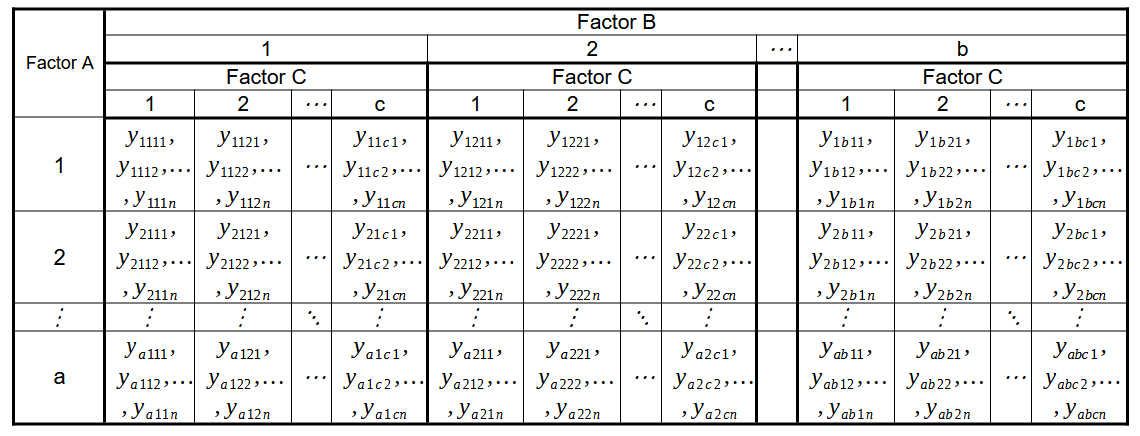
\includegraphics[width=0.90\linewidth]{img/factorial.png} 
	\caption{Disposición general para un diseño factorial con tres factores de efectos fijos.} 
	\label{fig:FactorialTres}
\end{figure}
\FloatBarrier

\textbf{El modelo para un diseño de tres factores es:}\\

\begin{center}
	$y_{ijkl}=\mu + \tau_{i} + \beta_{j} + \gamma_{k} + (\tau \beta)_{ij} +(\tau \gamma)_{ik} + (\beta \gamma)_{jk} + (\tau \beta \gamma)_{ijk} + \epsilon_{ijkl} $

	$i = 1,2, \dots, a$, $j = 1,2, \dots, b$, $k = 1,2, \dots, c$  y $l = 1,2, \dots, n$.
 \end{center}
 
Donde:
\begin{itemize}
	\item $\mu$ es la media general
	\item $\tau_{i}$ efecto del $i$-ésimo nivel del factor renglón $A$.
	\item $\beta_{j}$ efecto del $j$-ésimo nivel del factor columna $B$.
	\item $\gamma_{k} $ efecto del $k$-ésimo nivel del factor columna $C$.
	\item $(\tau \beta)_{ij} $ efecto de la interacción entre $\tau_{i}$  y  $\beta_{j}$ .
	\item $(\tau \gamma)_{ik}$ efecto de la interacción entre  $\tau_{i}$  y  $\gamma_{k}$ .
	\item $(\beta \gamma)_{jk}$ efecto de la interacción entre $\beta_{j}$ y  $\gamma_{k}$ .
	\item $(\tau \beta \gamma)_{ijk}$ efecto de la interacción entre $\tau_{i}$  , $\beta_{j}$ y $\gamma_{k}$ .
	\item $\epsilon_{ijkl}$ es el error aleatorio.
\end{itemize}


\textbf{Supuestos del modelo}\\

 $\epsilon_{ijkl} NI (0, \sigma^{2})$\\

\textbf{Hipótesis}\\

Para los factores:
\begin{center}
	$H^{1}_{0} =\tau_{1} = \tau_{2} = \dots = \tau_{a} = 0$ vs $H^{1}_{1}$ : al menos una $\tau_{i} \neq 0$ , $i = 1,2, \dots, a$ .\\
	$H^{2}_{0} =\beta_{1} = \beta_{2} = \dots = \beta_{b} = 0 $ vs $H^{2}_{1}$ : al menos una $\beta_{j} \neq 0$ , $j = 1,2, \dots,b$ .\\
	$H^{3}_{0} =\gamma_{1} = \gamma_{2} = \dots = \gamma_{c} = 0 $ vs $H^{3}_{1}$ : al menos una $\gamma_{k} \neq 0$ , $k = 1,2, \dots,c$ .\\
\end{center}

Para las interacciones:
\begin{center}
	$H^{4}_{0} : (\tau \beta)_{ij} = 0$ $ \forall i,j$ vs $H^{4}_{1}$ : al menos una $(\tau \beta)_{ij} \neq 0$ , $i = 1,2, \dots, a; j = 1,2, \dots,b$ .\\
	$H^{5}_{0} : (\tau \gamma)_{ik} = 0$ $ \forall i,k$ vs $H^{5}_{1}$ : al menos una $(\tau \gamma)_{ik} \neq 0$ , $i = 1,2, \dots, a; k = 1,2, \dots,c$ .\\
	$H^{6}_{0} : (\beta \gamma)_{jk} = 0$ $ \forall j,k$ vs $H^{6}_{1}$ : al menos una $(\beta \gamma)_{jk} \neq 0$ , $j = 1,2, \dots, b; k = 1,2, \dots, c$ .\\
	$H^{7}_{0} : (\tau \beta \gamma)_{ijk} = 0$ $ \forall i,j,k$ vs $H^{7}_{1}$ : al menos una $(\tau \beta \gamma)_{ijk} \neq 0$ , $i = 1,2, \dots, a; j = 1,2, \dots, b; k = 1,2, \dots, c$ .\\
\end{center}

\textbf{Suma de cuadrados}\\

Las fórmulas de cálculo para las sumas de cuadrados son:\\
{\large$ SC_{total} = \sum_{i=1}^{a}  \sum_{j=1}^{b}  \sum_{k=1}^{c}  \sum_{l=1}^{n} y_{ijkl}^{2} - \frac{y_{....}^{2}}{abcn} $} ,\\

{\large $ SC_{A} = \sum_{i=1}^{a} \frac{y_{i...}^{2}}{bcn}  - \frac{y_{....}^{2}}{abcn} $} ,\\

{\large$ SC_{B} = \sum_{j=1}^{b} \frac{y_{.j..}^{2}}{acn}  - \frac{y_{....}^{2}}{abcn} $}  ,\\

{\large$ SC_{C} = \sum_{k=1}^{c} \frac{y_{..k.}^{2}}{abn} - \frac{y_{....}^{2}}{abcn} $}.\\


\textbf{Las sumas de cuadrados para las interacciones son:}\\

{\large$ SC_{AB} = \sum_{i=1}^{a} \sum_{j=1}^{b}  \frac{y_{ij..}^{2}}{cn}  - \frac{y_{....}^{2}}{abcn} - SC_{A} -SC_{B} $}, \\

{\large$ SC_{AC} = \sum_{i=1}^{a} \sum_{k=1}^{c}  \frac{y_{i.k.}^{2}}{bn}  - \frac{y_{....}^{2}}{abcn} - SC_{A} -SC_{C} $}, \\

{\large$ SC_{BC} = \sum_{j=1}^{b} \sum_{k=1}^{c}  \frac{y_{.jk.}^{2}}{an}  - \frac{y_{....}^{2}}{abcn} - SC_{C} -SC_{B} $}, \\


$ SC_{ABC} =  \sum_{i=1}^{a}  \sum_{j=1}^{b}  \sum_{k=1}^{c}  \frac{y_{ijk.}^{2}}{n}  - \frac{y_{....}^{2}}{abcn} - SC_{A} -SC_{B} - SC_{C} -SC_{AB} -SC_{AC} -SC_{BC}  $ .\\


La suma de cuadrados del error puede encontrarse restando la suma de cuadrados de cada efecto principal e interacción de la suma de cuadrados total:\\

\begin{center}
	$ SC_{E} = SC_{T} -SC_{A} - SC_{B}-SC_{C} -SC_{AB} -SC_{AC} -SC_{BC} -SC_{ABC} $ .\\
\end{center}

O bien, 
\begin{center}
	$ SC_{E} = SC_{T} - SC_{Sub(ABC)} $,\\
\end{center}

donde
\begin{center}
$$ SC_{Sub(ABC)} = \sum_{i=1}^{a}  \sum_{j=1}^{b}  \sum_{k=1}^{c} \frac{y_{ijk.}^{2}}{n} - \frac{y_{....}^{2}}{abcn} .$$\\
\end{center}


\textbf{Estadísticos de prueba}\\

Para probar la significación la fuente de variabilidad $X$, se divide $CM_{X}$ por el  $CM_{E}$; de modo que los valores grandes de este cociente implican que los datos no apoyan la hipótesis nula correspondiente:
\begin{center}
	$ F^{X} = \frac{CM_{X}}{CM_{E}} \sim F_{x,abc(n-1)} $,\\
\end{center}


donde $x$ representa los grados de libertad asociados a la fuente de variabilidad $X$.\\

\textbf{Región de rechazo}\\

Con un nivel de significación dado $\alpha$, la región de rechazo se encuentra en la cola superior de la distribución F correspondiente:

\begin{center}
	$ RR : F_{0}^{X} > F_{a;x,abc(n-1)} $,\\
\end{center}

donde $F_{0}^{X} $ es el valor de la estadística de prueba correspondiente.\\

\textbf{Valor p}\\

Se considera la fuente de variación $(X)$ con su correspondiente estadístico de prueba:

\begin{center}
	$ P_{X} =  P( F_{a;x,abc(n-1)} \geq F_{0}^{X} ) $.\\
\end{center}


\begin{table}[ht]
	\centering
	\begin{tabular}{|c|c|c|c|c|c|}
		\hline
		\makecell{Fuente de \\ variación} & SC & g.l & CM & $F_{0}$ & Valor - p \\ % Encabezados de columna
		\hline
		A & $SC_{A}$ & $a-1$ & $\frac{SC_{A}}{a-1}$ &  $\frac{CM_{A}}{CM_{E}}$ & $P(F \geq F_{0}^{A} )$ \\
		\hline
		B & $SC_{B}$ & $b-1$ & $\frac{SC_{B}}{b-1}$ &  $\frac{CM_{B}}{CM_{E}}$ & $P(F \geq F_{0}^{B} )$ \\
		\hline
		C & $SC_{C}$ & $c-1$ & $\frac{SC_{C}}{c-1}$ &  $\frac{CM_{C}}{CM_{E}}$ & $P(F \geq F_{0}^{C} )$ \\
		\hline
		AB & $SC_{AB}$ & $(a-1)(b-1)$ & $\frac{SC_{AB}}{(a-1)(b-1)}$ &  $\frac{CM_{AB}}{CM_{E}}$ & $P(F \geq F_{0}^{AB} )$ \\
		\hline
		AC & $SC_{AC}$ & $(a-1)(c-1)$ & $\frac{SC_{AC}}{(a-1)(c-1)}$ &  $\frac{CM_{AC}}{CM_{E}}$ & $P(F \geq F_{0}^{AC} )$ \\
		\hline
		BC & $SC_{BC}$ & $(b-1)(c-1) $ & $\frac{SC_{BC}}{(b-1)(c-1)}$ &  $\frac{CM_{BC}}{CM_{E}}$ & $P(F \geq F_{0}^{BC} )$ \\
		\hline
		ABC & $SC_{ABC}$ & $(a-1)(b-1)(c-1)$ & $\frac{SC_{ABC}}{(a-1)(b-1)(c-1)}$ &  $\frac{CM_{ABC}}{CM_{E}}$ & $P(F \geq F_{0}^{ABC} )$ \\
		\hline
		Error & $SC_{E} $ & $abc(n-1)$ & $\frac{SC_{E}}{abc(n-1)}$ & & \\
		\hline
		Total & $SC_{T}$ & $abcn-1$ & & &  \\
		\hline
	\end{tabular}
	\caption{Tabla del ANOVA para el diseño factorial de tres factores con efectos fijos.}
\end{table}
\FloatBarrier

\subsubsection{Comparación múltiple de Tukey \parencite{montgomery-2017}}

Si el ANOVA indica que hay diferencia en el nivel medio de los factores resulta de interés llevar a cabo comparaciones entre las medias individuales para determinar diferencias específicas. Existiendo interacción significativa, los efectos de los factores no son independientes.\\


Con la prueba de Tukey el nivel de significación global es exactamente  cuando los tamaños de las muestras son iguales y como máximo $\alpha$ cuando los tamaños de las muestras son desiguales. Este método también puede utilizarse para construir intervalos de confianza sobre las diferencias en todos los pares de medias. Para estos intervalos, el nivel de confianza simultáneo es del $(1-\alpha)100\%$ cuando los tamaños de las muestras son iguales y de al menos $(1-\alpha)100\%$  cuando los tamaños de las muestras son desiguales.\\
%%%Revisar acentos

$H_{0}:\mu_{i} = \mu_{j}$ vs $H_{1}:\mu_{i} \neq \mu_{j}$ para toda $i \neq j$.\\

 $\mu_{i} \neq \mu_{j}$ si $| \bar{Y}_{i} -\bar{Y}_{j} | > q_{\alpha} (p,f) \: \sqrt{\frac{CM_{E}}{n}} = T_{\alpha}$ (tamaños de las muestras iguales).\\
 

La tabla V del apéndice en \textcite{montgomery-2017} contiene $q_{\alpha} (p,f)$, valor del punto porcentual $\alpha$ superior del estadístico del rango estudentizado {\large $q=\frac{ \bar{Y}_{max} -\bar{Y}_{min}}{ \sqrt{\frac{CM_{E}}{n}}}$}, donde $\bar{Y}_{max}$ y $\bar{Y}_{min}$ son las medias muestrales mayor y menor respectivamente de un grupo de $p$ medias muestrales, $f$ son los gl asociados con $CM_{E}$.\\
 
Con intervalo de confianza del  $(1-\alpha)100\%$ para $\mu_{i} - \mu_{j}$:\\
 
\begin{center}
	$ \bar{Y}_{max} -\bar{Y}_{min} -  q_{\alpha} (p,f) \: \sqrt{\frac{CM_{E}}{n}} \leq \mu_{i} - \mu_{j} \leq \bar{Y}_{max} -\bar{Y}_{min} + q_{\alpha} (p,f) \: \sqrt{\frac{CM_{E}}{n}} $. \\
\end{center}

Para tamaños de muestras desiguales, en la prueba de hipótesis se utiliza:\\

\begin{center}
	$$ T_{\alpha} = \frac{q_{\alpha} (p,f)}{\sqrt{2}} \sqrt{CM_{E} (\frac{1}{n_{i}} + \frac{1}{n_{j}})}  .$$ \\
\end{center}


Los intervalos de confianza para la diferencia de los pares de medias se determinan con:\\


\begin{center}
	$ \bar{Y}_{max} -\bar{Y}_{min} -  \frac{q_{\alpha} (p,f)}{\sqrt{2}} \sqrt{CM_{E} (\frac{1}{n_{i}} + \frac{1}{n_{j}})}  \leq \mu_{i} - \mu_{j} \leq \bar{Y}_{max} -\bar{Y}_{min} + \frac{q_{\alpha} (p,f)}{\sqrt{2}} \sqrt{CM_{E} (\frac{1}{n_{i}} + \frac{1}{n_{j}})}  $. \\
\end{center}

Donde la versión para tamaños de las muestras diferentes se llama el procedimiento de Tukey-Kramer.
